% Experiment workflow, from setup to the report.
% Build: pdflatex workflow.tex, then render the PDF to ../workflow.png
\documentclass[border=6pt]{standalone}
\usepackage[T1]{fontenc}
\usepackage{helvet}
\renewcommand{\familydefault}{\sfdefault}
\usepackage{tikz}
\usetikzlibrary{arrows.meta,positioning,fit,backgrounds,calc}
\definecolor{acc}{HTML}{1F4E8C}
\definecolor{acc2}{HTML}{2F7BBF}
\definecolor{s1}{HTML}{EAF2FC}
\definecolor{s2}{HTML}{FFF4E5}
\definecolor{s3}{HTML}{ECF7EF}
\definecolor{s4}{HTML}{F6EAF3}
\definecolor{kh}{HTML}{B35C00}
\begin{document}
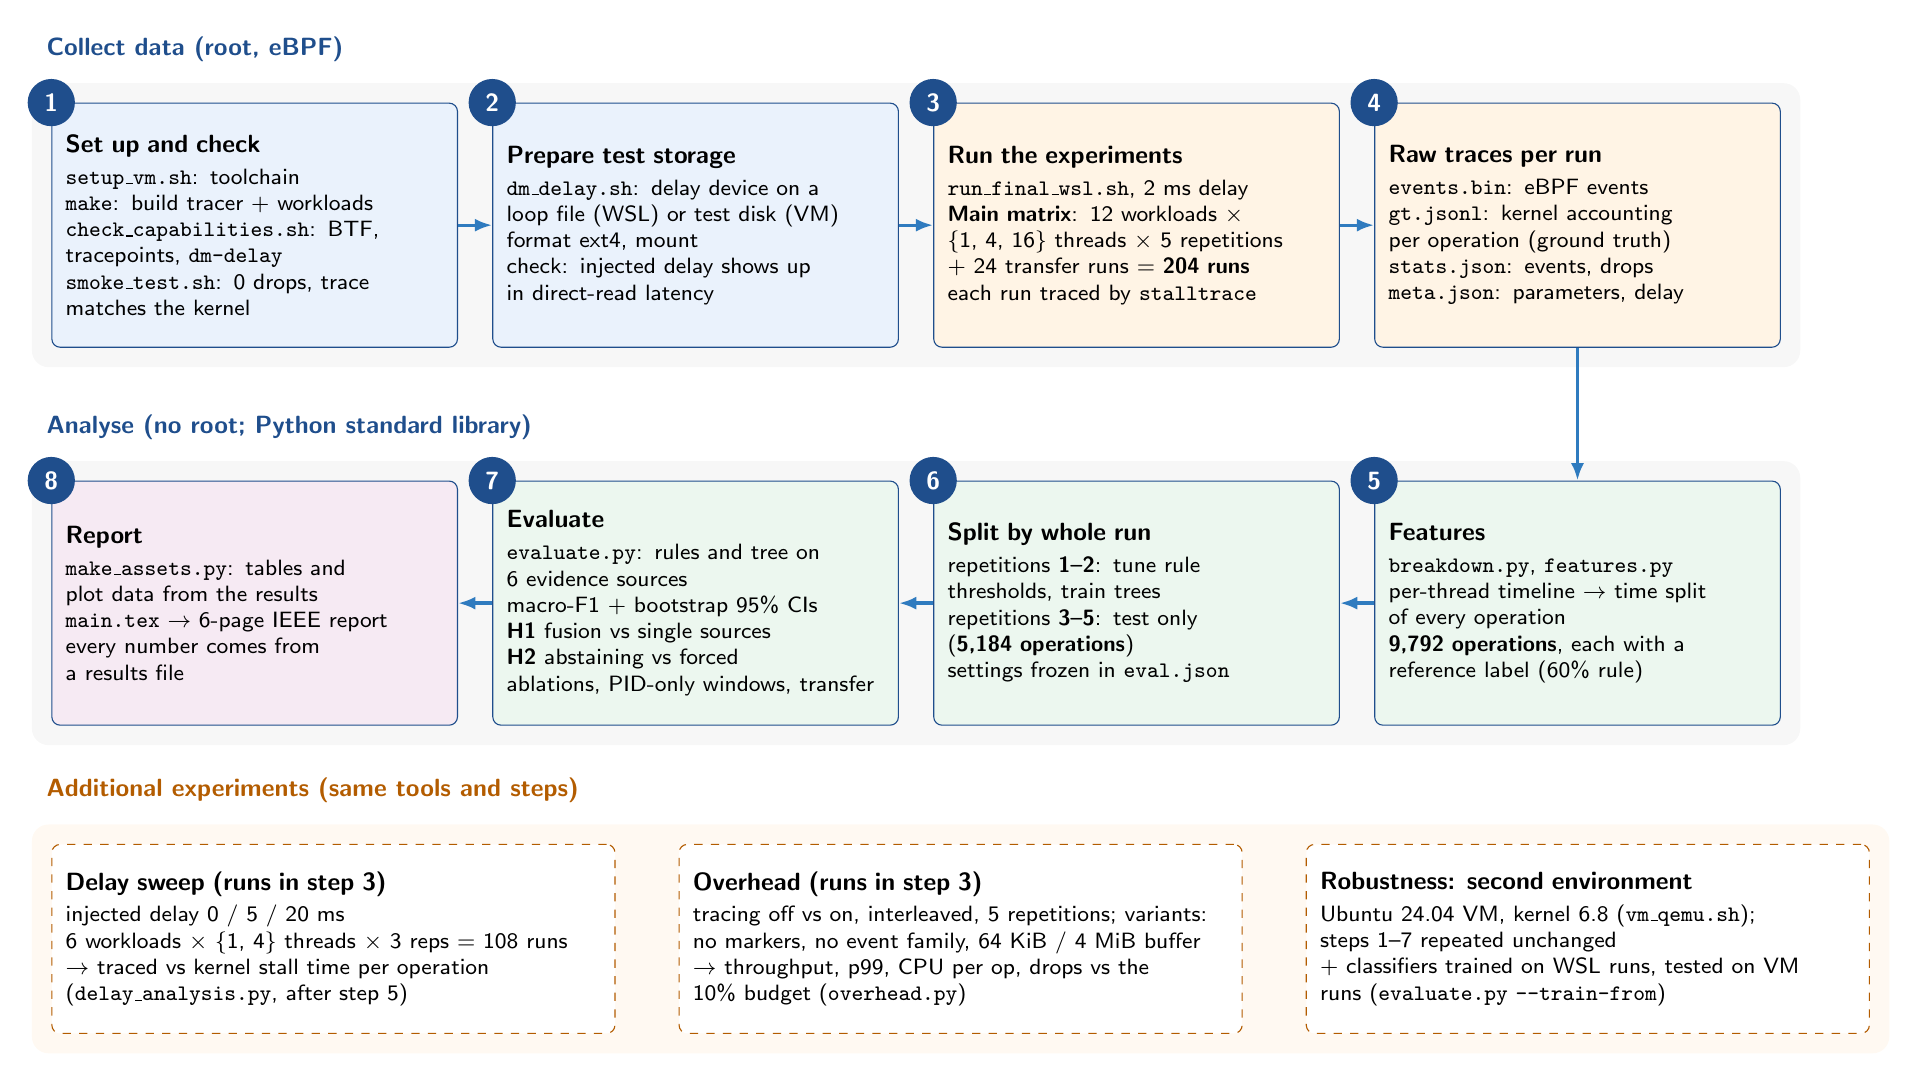
\begin{tikzpicture}[font=\footnotesize, >={Latex[length=2.2mm]},
  every node/.append style={execute at begin node={\hyphenpenalty=10000\exhyphenpenalty=10000}},
  stage/.style={draw=acc, rounded corners=3pt, align=left, inner sep=5pt, text width=48mm,
               minimum height=31mm, anchor=north},
  num/.style={circle, fill=acc, text=white, font=\bfseries\small, inner sep=1.5pt, minimum size=6mm},
  arr/.style={->, very thick, acc2},
  side/.style={draw=kh, dashed, rounded corners=3pt, align=left, inner sep=5pt, text width=46mm, fill=white},
  cmd/.style={font=\scriptsize\ttfamily}]

\newcommand{\head}[1]{{\bfseries\small #1}\\[2pt]}

% ---- row 1: preparation and data collection
\node[stage, fill=s1] (a) at (0,0) {\head{Set up and check}
  \texttt{setup\_vm.sh}: toolchain\\
  \texttt{make}: build tracer + workloads\\
  \texttt{check\_capabilities.sh}: BTF,\\tracepoints, \texttt{dm-delay}\\
  \texttt{smoke\_test.sh}: 0 drops, trace\\matches the kernel};
\node[stage, fill=s1] (b) at (5.6,0) {\head{Prepare test storage}
  \texttt{dm\_delay.sh}: delay device on a\\loop file (WSL) or test disk (VM)\\
  format ext4, mount\\
  check: injected delay shows up\\in direct-read latency};
\node[stage, fill=s2] (c) at (11.2,0) {\head{Run the experiments}
  \texttt{run\_final\_wsl.sh}, 2 ms delay\\
  \textbf{Main matrix}: 12 workloads $\times$\\\{1, 4, 16\} threads $\times$ 5 repetitions\\+ 24 transfer runs = \textbf{204 runs}\\
  each run traced by \texttt{stalltrace}};
\node[stage, fill=s2] (d) at (16.8,0) {\head{Raw traces per run}
  \texttt{events.bin}: eBPF events\\
  \texttt{gt.jsonl}: kernel accounting\\per operation (ground truth)\\
  \texttt{stats.json}: events, drops\\
  \texttt{meta.json}: parameters, delay};

% ---- row 2: analysis
\node[stage, fill=s3] (e) at (16.8,-4.8) {\head{Features}
  \texttt{breakdown.py}, \texttt{features.py}\\
  per-thread timeline $\rightarrow$ time split\\of every operation\\
  \textbf{9,792 operations}, each with a\\reference label (60\% rule)};
\node[stage, fill=s3] (f) at (11.2,-4.8) {\head{Split by whole run}
  repetitions \textbf{1--2}: tune rule\\thresholds, train trees\\
  repetitions \textbf{3--5}: test only\\(\textbf{5,184 operations})\\
  settings frozen in \texttt{eval.json}};
\node[stage, fill=s3] (g) at (5.6,-4.8) {\head{Evaluate}
  \texttt{evaluate.py}: rules and tree on\\6 evidence sources\\
  macro-F1 + bootstrap 95\% CIs\\
  \textbf{H1} fusion vs single sources\\
  \textbf{H2} abstaining vs forced\\
  ablations, PID-only windows, transfer};
\node[stage, fill=s4] (h) at (0,-4.8) {\head{Report}
  \texttt{make\_assets.py}: tables and\\plot data from the results\\
  \texttt{main.tex} $\rightarrow$ 6-page IEEE report\\
  every number comes from\\a results file};

% numbers
\foreach \n/\k in {a/1,b/2,c/3,d/4,e/5,f/6,g/7,h/8}
  \node[num] at (\n.north west) {\k};

% main flow
\draw[arr] (a.east) -- (b.west);
\draw[arr] (b.east) -- (c.west);
\draw[arr] (c.east) -- (d.west);
\draw[arr] (d.south) -- (e.north);
\draw[arr] (e.west) -- (f.east);
\draw[arr] (f.west) -- (g.east);
\draw[arr] (g.west) -- (h.east);

% ---- additional experiments: same pipeline, own band, no crossing arrows
\node[side, text width=68mm, minimum height=24mm, anchor=north west] (sw) at ($(h.south west)+(0,-15mm)$)
  {\head{Delay sweep (runs in step 3)}
  injected delay 0 / 5 / 20 ms\\6 workloads $\times$ \{1, 4\} threads $\times$ 3 reps = 108 runs\\
  $\rightarrow$ traced vs kernel stall time per operation\\(\texttt{delay\_analysis.py}, after step 5)};
\node[side, text width=68mm, minimum height=24mm, right=8mm of sw] (ov)
  {\head{Overhead (runs in step 3)}
  tracing off vs on, interleaved, 5 repetitions; variants:\\no markers, no event family, 64 KiB / 4 MiB buffer\\
  $\rightarrow$ throughput, p99, CPU per op, drops vs the\\10\% budget (\texttt{overhead.py})};
\node[side, text width=68mm, minimum height=24mm, right=8mm of ov] (vm)
  {\head{Robustness: second environment}
  Ubuntu 24.04 VM, kernel 6.8 (\texttt{vm\_qemu.sh});\\steps 1--7 repeated unchanged\\
  + classifiers trained on WSL runs, tested on VM\\runs (\texttt{evaluate.py -{}-train-from})};

\begin{scope}[on background layer]
  \node[rounded corners=6pt, fill=gray!6, inner sep=7pt, fit=(a)(d)] (R1) {};
  \node[rounded corners=6pt, fill=gray!6, inner sep=7pt, fit=(e)(h)] (R2) {};
  \node[rounded corners=6pt, fill=orange!5, inner sep=7pt, fit=(sw)(vm)] (R3) {};
\end{scope}
\node[font=\bfseries\small, text=acc, anchor=south west] at ($(R1.north west)+(2pt,4pt)$) {Collect data (root, eBPF)};
\node[font=\bfseries\small, text=acc, anchor=south west] at ($(R2.north west)+(2pt,4pt)$) {Analyse (no root; Python standard library)};
\node[font=\bfseries\small, text=kh, anchor=south west] at ($(R3.north west)+(2pt,4pt)$) {Additional experiments (same tools and steps)};
\end{tikzpicture}
\end{document}
